\documentclass{article}\usepackage[]{graphicx}\usepackage[]{color}
%% maxwidth is the original width if it is less than linewidth
%% otherwise use linewidth (to make sure the graphics do not exceed the margin)
\makeatletter
\def\maxwidth{ %
  \ifdim\Gin@nat@width>\linewidth
    \linewidth
  \else
    \Gin@nat@width
  \fi
}
\makeatother

\definecolor{fgcolor}{rgb}{0.345, 0.345, 0.345}
\newcommand{\hlnum}[1]{\textcolor[rgb]{0.686,0.059,0.569}{#1}}%
\newcommand{\hlstr}[1]{\textcolor[rgb]{0.192,0.494,0.8}{#1}}%
\newcommand{\hlcom}[1]{\textcolor[rgb]{0.678,0.584,0.686}{\textit{#1}}}%
\newcommand{\hlopt}[1]{\textcolor[rgb]{0,0,0}{#1}}%
\newcommand{\hlstd}[1]{\textcolor[rgb]{0.345,0.345,0.345}{#1}}%
\newcommand{\hlkwa}[1]{\textcolor[rgb]{0.161,0.373,0.58}{\textbf{#1}}}%
\newcommand{\hlkwb}[1]{\textcolor[rgb]{0.69,0.353,0.396}{#1}}%
\newcommand{\hlkwc}[1]{\textcolor[rgb]{0.333,0.667,0.333}{#1}}%
\newcommand{\hlkwd}[1]{\textcolor[rgb]{0.737,0.353,0.396}{\textbf{#1}}}%
\let\hlipl\hlkwb

\usepackage{framed}
\makeatletter
\newenvironment{kframe}{%
 \def\at@end@of@kframe{}%
 \ifinner\ifhmode%
  \def\at@end@of@kframe{\end{minipage}}%
  \begin{minipage}{\columnwidth}%
 \fi\fi%
 \def\FrameCommand##1{\hskip\@totalleftmargin \hskip-\fboxsep
 \colorbox{shadecolor}{##1}\hskip-\fboxsep
     % There is no \\@totalrightmargin, so:
     \hskip-\linewidth \hskip-\@totalleftmargin \hskip\columnwidth}%
 \MakeFramed {\advance\hsize-\width
   \@totalleftmargin\z@ \linewidth\hsize
   \@setminipage}}%
 {\par\unskip\endMakeFramed%
 \at@end@of@kframe}
\makeatother

\definecolor{shadecolor}{rgb}{.97, .97, .97}
\definecolor{messagecolor}{rgb}{0, 0, 0}
\definecolor{warningcolor}{rgb}{1, 0, 1}
\definecolor{errorcolor}{rgb}{1, 0, 0}
\newenvironment{knitrout}{}{} % an empty environment to be redefined in TeX

\usepackage{alltt}
\usepackage{graphicx, color, hyperref, fancyhdr}

%\input{../brayTeachingStyle}

\usepackage[top=.5in, bottom=.5in, left=1.1in, right=1.1in]{geometry}
\thispagestyle{empty}
\IfFileExists{upquote.sty}{\usepackage{upquote}}{}
\begin{document}

\begin{center}
\textsc{CMSC 205: Data-Scientific Programming} \\
\noindent\rule{12cm}{0.4pt}
\end{center}


\begin{enumerate}
\setlength\itemsep{4em}

\item The plot below represents the predictor space (on $X_1$ and $X_2$) with a training data set plotted and the class of their response variable indicated by the color.

\begin{minipage}{.5\linewidth}
{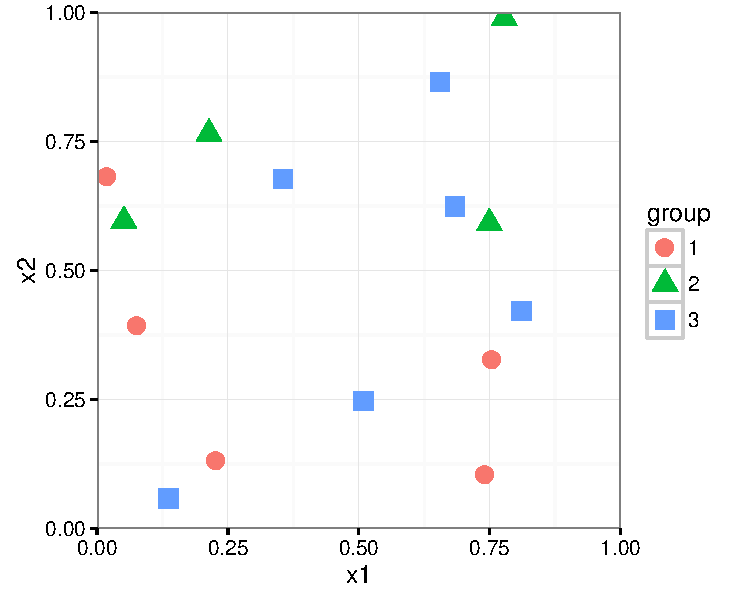
\includegraphics[scale=0.6]{3-class-plot}}
\end{minipage}
\begin{minipage}{.5\linewidth}

\begin{enumerate}
\setlength\itemsep{3em}
\item If we consider this a classification tree without any splits yet (i.e. only one region), what would be the prediction for \emph{every} new observation?
\item What is the (training) misclassification rate?
\item What is the GINI index?
% \item What is the cross-entropy?
\end{enumerate}

\end{minipage}

\item Add a straight line, parallel to one of the axes, that splits the predictor space into two regions. Choose the split in a way that you think will lead to the best overall improvement in the metrics above. Label the new regions $\textrm{R}_1$ and $\textrm{R}_2$ and calculate the metrics for each.

\vspace{5mm}

\begin{minipage}{.5\linewidth}
\begin{center}
$\textrm{R}_1$
\end{center}
\begin{enumerate}
\setlength\itemsep{3em}
\item What is the predicted class?
\item What is the misclassification rate?
\item What is the GINI index?
% \item What is the cross-entropy?
\end{enumerate}
\end{minipage}
\begin{minipage}{.5\linewidth}
\begin{center}
$\textrm{R}_2$
\end{center}
\begin{enumerate}
\setlength\itemsep{3em}
\item What is the predicted class?
\item What is the misclassification rate?
\item What is the GINI index?
% \item What is the cross-entropy?
\end{enumerate}

\end{minipage}
\item To decide if the split in Q2 was optimal, we need to evaluate how much the metrics in Q1 have improved. This requires combining the metrics across $\textrm{R}_1$ and $\textrm{R}_2$ in Q2. Please do so in a sensible way so that you can answer: what was the overall decrease each metric going from one region/node to two?

Misclassification: \hspace{30mm} GINI: %\hspace{30mm} Cross-entropy:

\vspace{5mm}

\item On the back of this page, please draw the (very simple) tree corresponding to your partition.

\end{enumerate}

\end{document}
